\documentclass[10pt, a4paper]{scrartcl}

\usepackage{vorschule}
\usepackage[
	typ=ab,
	fach=Informatik,
	lerngruppe={9Diff},
	nummer={II.3},
	module={Symbole,Lizenzen},
	seitenzahlen=keine,
	farbig,
	lizenz=cc-by-nc-sa-4,
]{schule}

\usepackage[
	kuerzel=Ngb,
	reihe={Informationen, Daten und Codierung},
	version={2020-09-02},
]{ngbschule}

\author{J. Neugebauer}
\title{Binärzahlen}
\date{\Heute}

\setzeAufgabentemplate{ngbnormal}

\begin{document}
\ReiheTitel

Ein \emph{Zahlensystem} ist ein System zur Darstellung von Zahlen. Wir benutzen im Alltag das \emph{Dezimalsystem}, ein sogenanntes \emph{Stellenwertsystem} zur Basis 10. Das bedeutet, es werden 10 verschiedene Ziffern zur Darstellung benutzt. Das \emph{Binärsystem} benutzt nur zwei, und das \emph{Hexadezimalsystem} verwendet ganze 16.

Die Berechnung des Zahlwertes einer Binärzahl im Dezimalsystem erfolgt nach der Formel
\[ (1100111)_2 = 1\cdot 2^6 + 1\cdot 2^5 + 0\cdot 2^4 + 0\cdot 2^3 + 1\cdot 2^2 + 1\cdot 2^1 + 1\cdot 2^0 = (103)_{10} \]

\begin{aufgabe}[symbol=\Large\symHeft]
	Rechne in das Dezimalsystem um.
	\begin{tasks}(3)
		\task $(1101)_2$
		\task $(1000 0001)_2$
		\task $(1001 1111)_2$
	\end{tasks}
\end{aufgabe}

\begin{aufgabe}[symbol=\Large\symHeft\yspace\symPartner]
	Rechne in das Binärsystem um. Nutze jeweils das \emph{Subtraktions-} und das \emph{Moduloverfahren}. Diskutiere dann mit deinem Sitznachbarn, welches Verfahren in welcher Situation besser geeignet ist.
	\begin{tasks}(3)
		\task $(65)_{10}$
		\task $(71)_{10}$
		\task $(1000)_{10}$
	\end{tasks}
\end{aufgabe}

\begin{aufgabe}[symbol=\Large\symLaptop\yspace\symPartner]
	Erstellt in \programm{Scratch} ein Programm, dass eine Dezimalzahl mit dem Moduloverfahren in eine Binärzahl umrechnen kann. Nutze dazu die folgende Vorlage und ersetze die fehlenden Befehle (durch \code{xxx} markiert) mit den passenden Blöcken aus dem Bereich \enquote{Variablen}.
	\begin{center}
	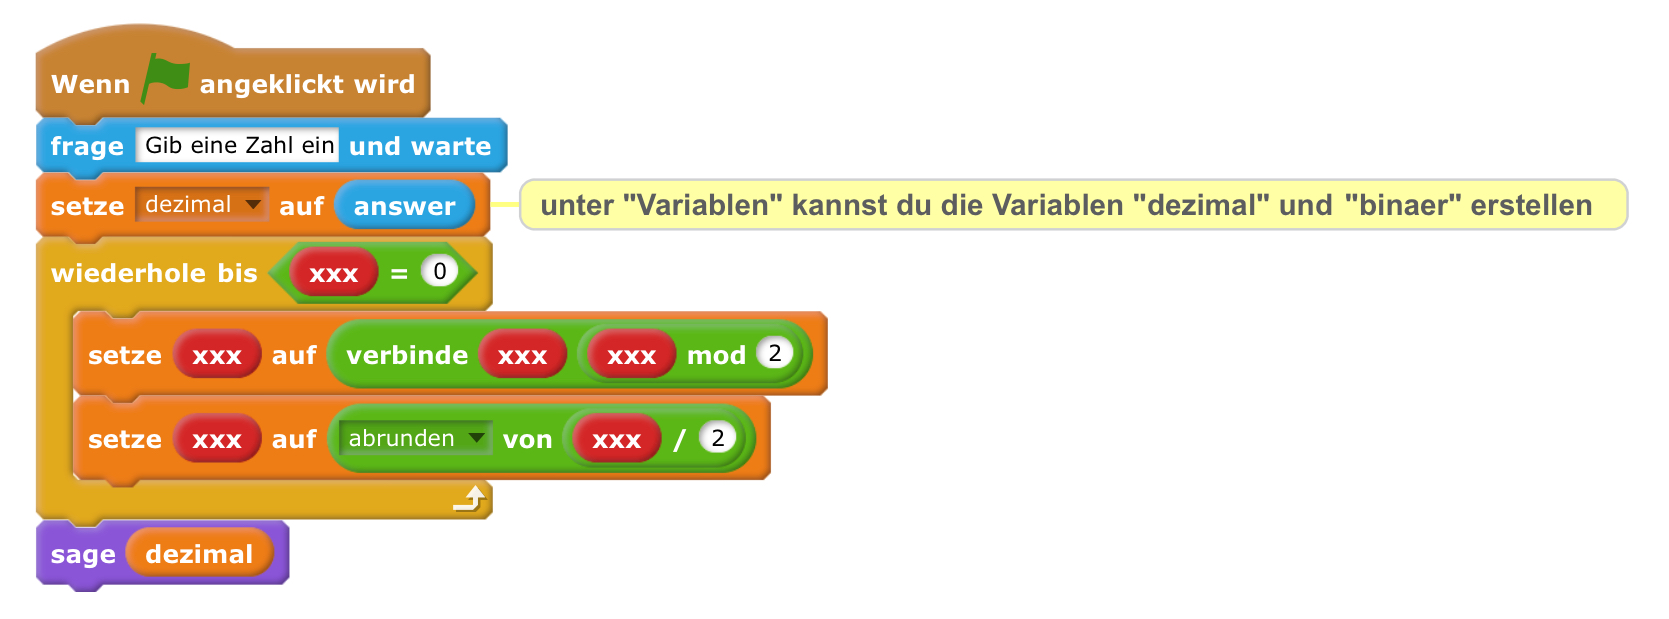
\includegraphics[width=8cm]{9Diff-AB.II.3-Abb_ScratchDezBin}
	\end{center}
\end{aufgabe}

\end{document}
